This section includes additional experimental results.
\paragraph{Sudoku:}
For the Sudoku experiments, this section presents additional results from different measurements.

\begin{figure}[H]
    \centering
    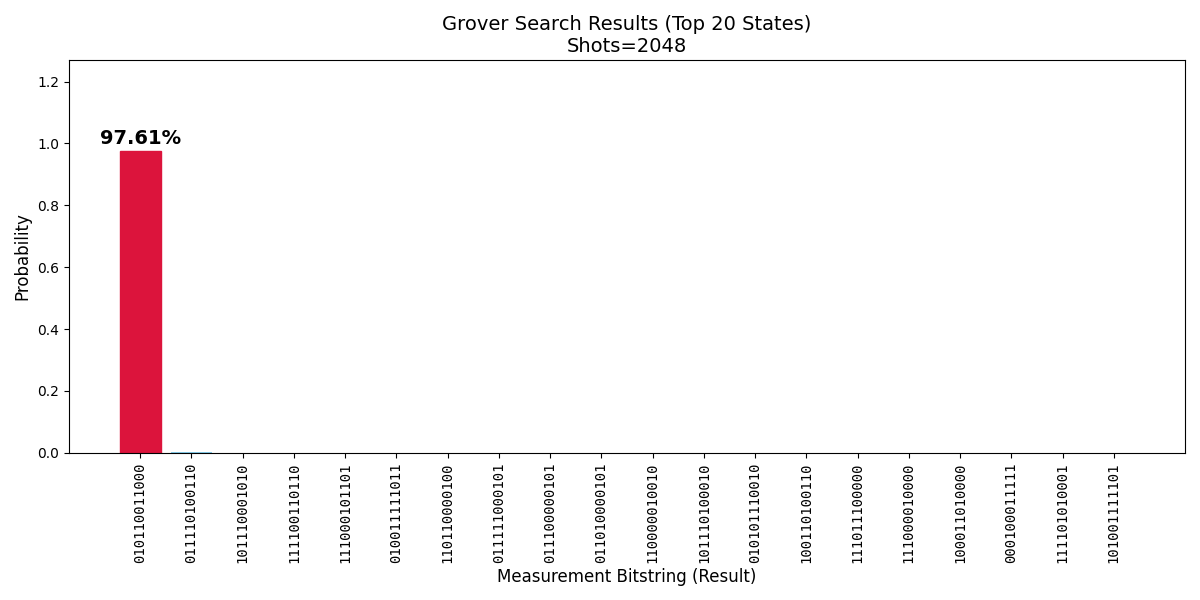
\includegraphics[width=1\linewidth]{SIMULATOR_3.png}
    \caption{Simulation results for 45 iterations showing 97.61\% probability.}
    \label{fig:sim_45} 
\end{figure}

\begin{figure}[H]
    \centering
    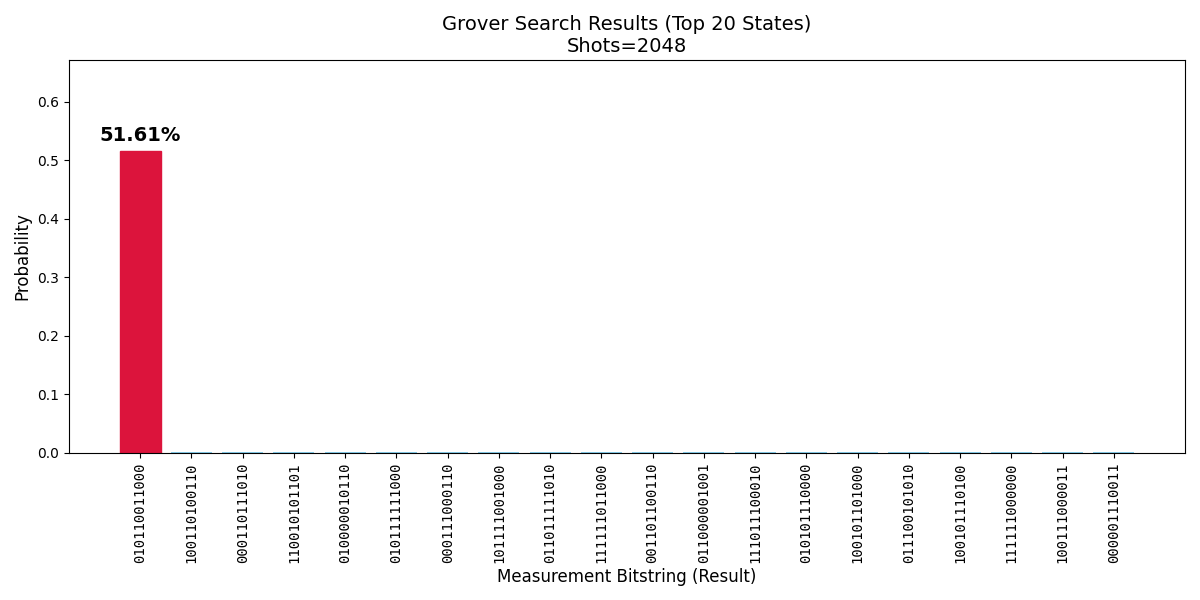
\includegraphics[width=1\linewidth]{Figure_12.png}
    \caption{Simulation results for 25 iterations showing 51.61\% probability.}
    \label{fig:sim_25}
\end{figure}

\begin{figure}[H]
    \centering
    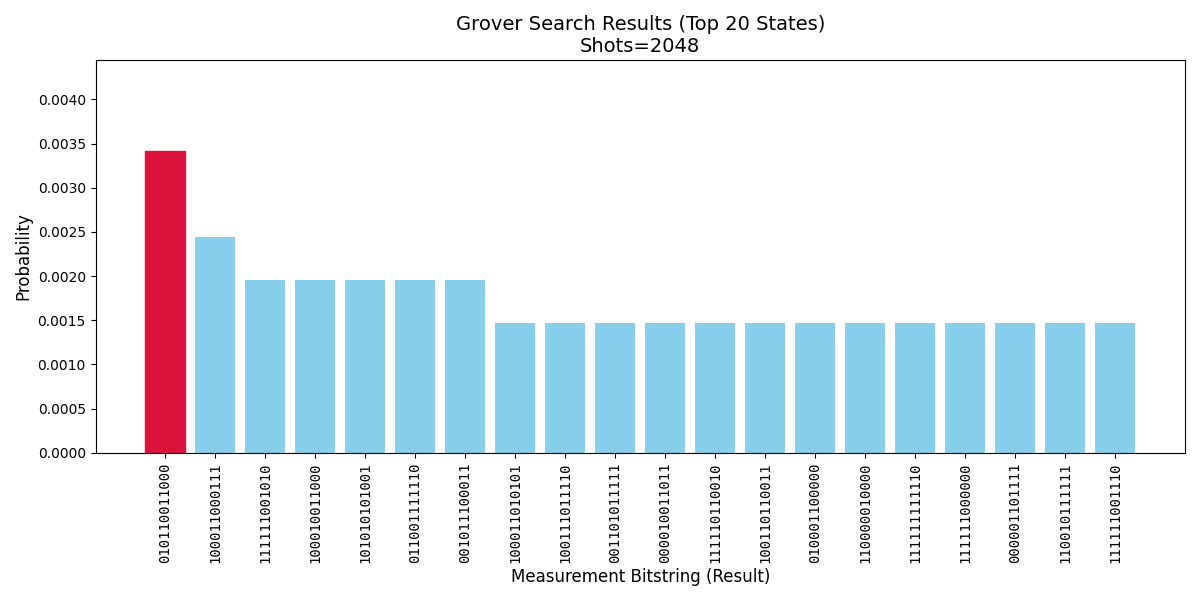
\includegraphics[width=1\linewidth]{Figure_12112.png}
    \caption{Simulation results for one iteration showing $\sim0.0035\%$ probability.}
    \label{fig:sim_1}
\end{figure}

\paragraph{WFC:}
For the Wave Function Collapse method, this section presents additional map generations and graphs for different grid sizes.

\begin{figure}[H]
  \centering
  \subfloat[Generated map A]{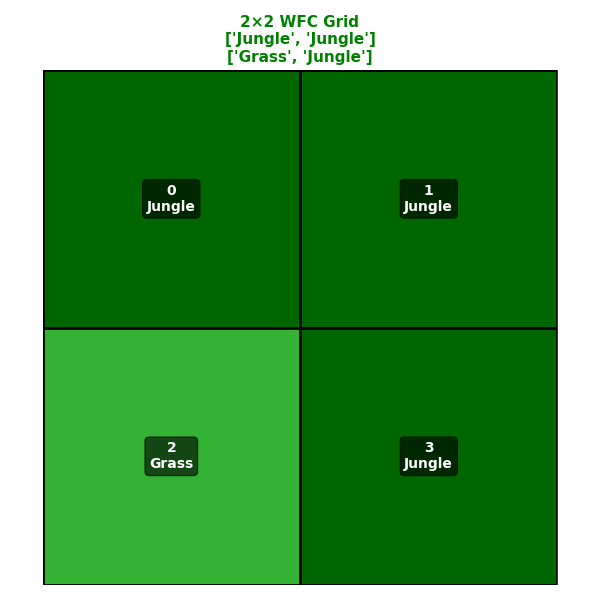
\includegraphics[width=0.5\linewidth]{figures/wfc/Figure_1_2x2.png}\label{fig:f1}}
  \hfill
  \subfloat[Generated map B]{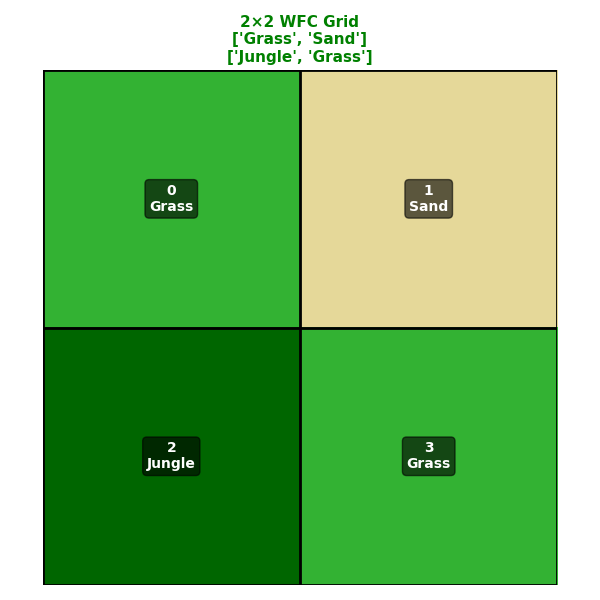
\includegraphics[width=0.5\linewidth]{figures/wfc/Figure_2_2x2.png}\label{fig:f2}}
  \caption{2$\times$2 maps generated using the quantum Wave Function Collapse (WFC) method with Aer.}
  \label{fig:quantum_wfc_2x2}
\end{figure}

\begin{figure}[H]
  \centering
  \subfloat[Generated map A]{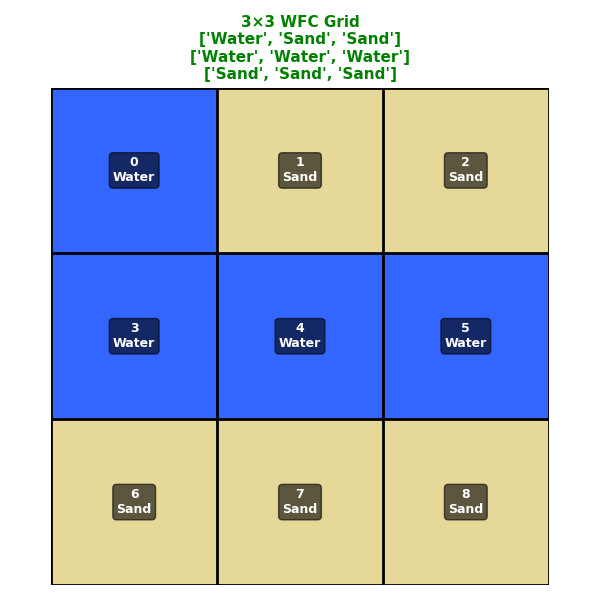
\includegraphics[width=0.5\linewidth]{figures/wfc/Figure_2.png}\label{fig:f1}}
  \hfill
  \subfloat[Generated map B]{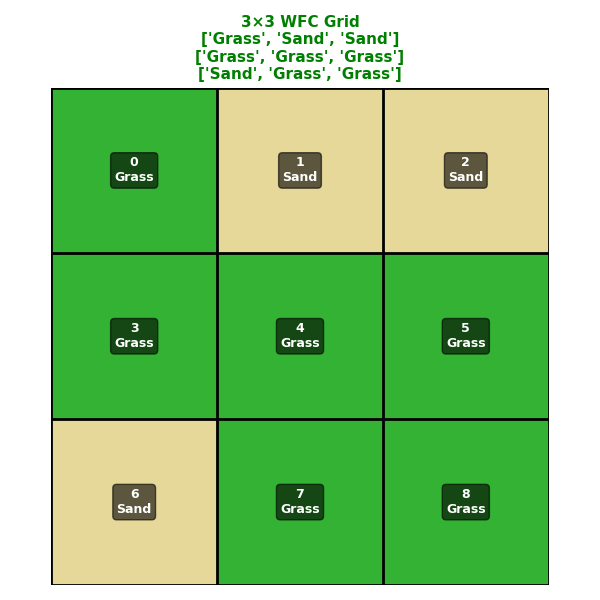
\includegraphics[width=0.5\linewidth]{figures/wfc/Figure_7.png}\label{fig:f2}}
  \caption{3$\times$3 maps generated using the quantum Wave Function Collapse (WFC) method with Aer.}
  \label{fig:quantum_wfc_3x3}
\end{figure}

\begin{figure}[H]
    \centering
    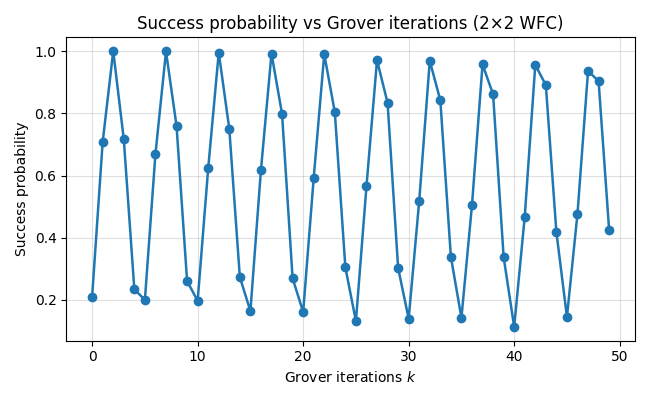
\includegraphics[width=0.6\textwidth]{figures/wfc/Figure_4.png}
    \caption{Probability of obtaining a valid 2$\times$2 map as a function of the number of Grover iterations. The success probability follows the characteristic quadratic sinusoidal behavior of Grover’s algorithm.}
    \label{fig:wfc_2x2_probability}
\end{figure}

\begin{figure}[H]
    \centering
    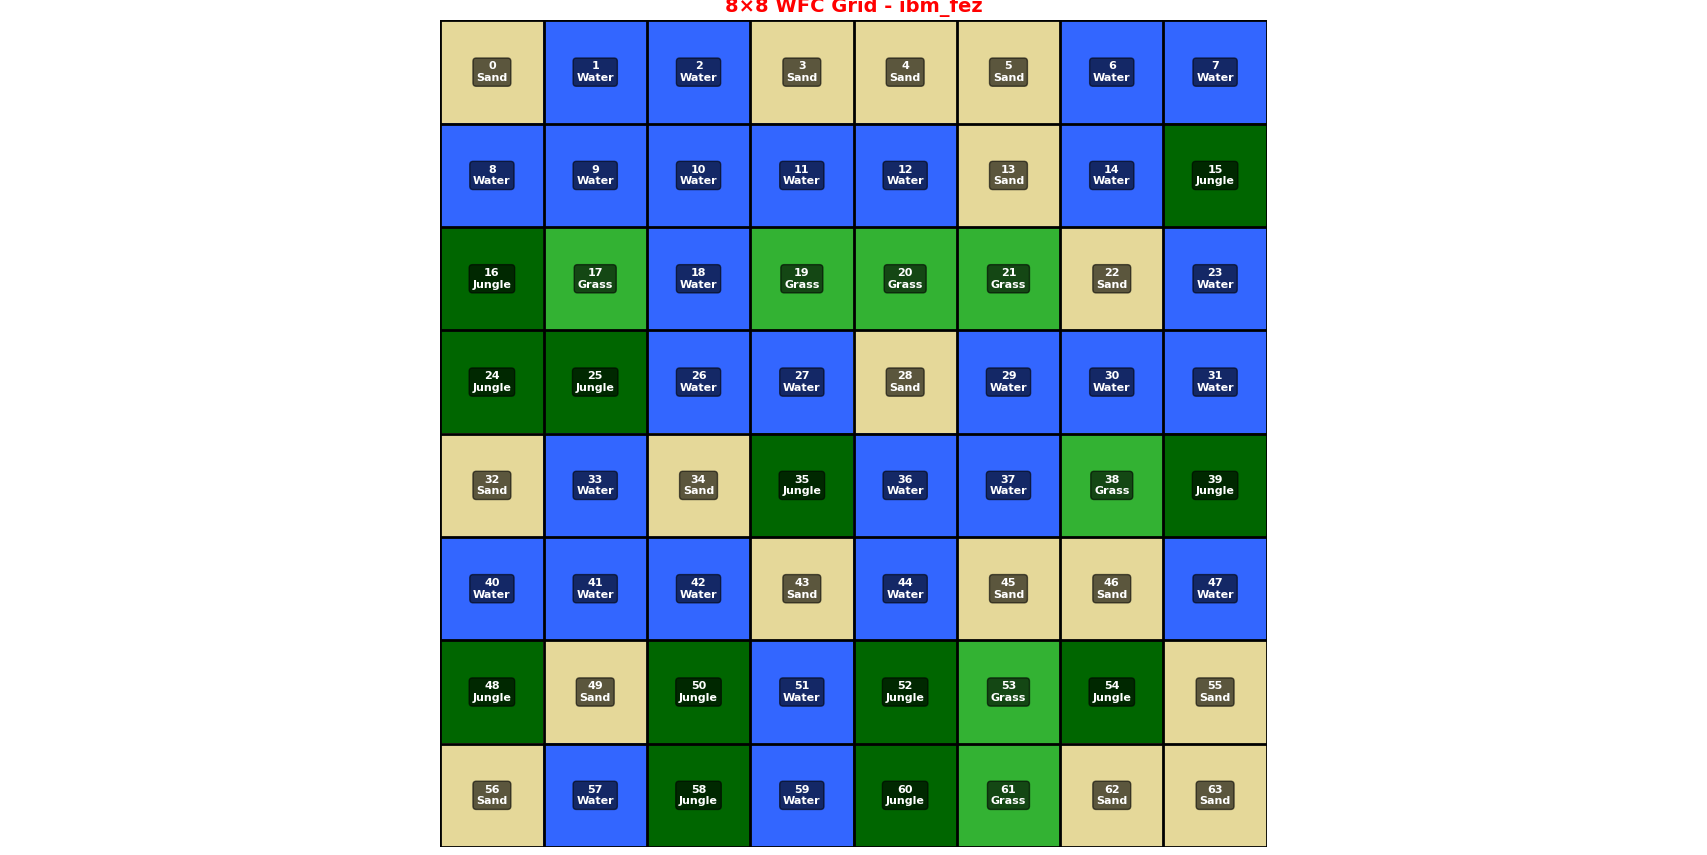
\includegraphics[width=1\textwidth]{figures/wfc/Figure_1.png}
    \caption{8$\times$8 map (largest possible map to generate) using the quantum Wave Function Collapse (WFC) method with IBM hardware.}
    \label{fig:quantum_wfc_8x8}
\end{figure}







